% questions.tex —— 2010 年·普通高等学校招生考试·江西卷·文科 · 题目内容片段（无答案）
% 由 tools/generate_projects.py 依来源总账自 2010/2010_数学真题_江西文_试题.md 生成，勿手改（改源 MD 后重跑）


状态：needs-review；依固定候选 PDF 两页（印刷页 609–610）逐题核验，五幅图已矢量重绘。原页未印分值，不补。

\gkpart{一、选择题}

\begin{question}
\gkti{1}对于实数 $a,b,c$，“$a>b$”是“$ac^2>bc^2$”的（　）

（A）充分不必要条件

（B）必要不充分条件

（C）充要条件

（D）既不充分也不必要条件

\end{question}
\begin{question}
\gkti{2}若集合 $A=\{x\mid |x|\leqslant1\}$，$B=\{x\mid x\geqslant0\}$，则 $A\cap B=$（　）

（A）$\{x\mid -1\leqslant x\leqslant1\}$

（B）$\{x\mid x\geqslant0\}$

（C）$\{x\mid 0\leqslant x\leqslant1\}$

（D）$\varnothing$

\end{question}
\begin{question}
\gkti{3}$(1-x)^{10}$ 展开式中 $x^3$ 项的系数为（　）

（A）$-720$

（B）$720$

（C）$120$

（D）$-120$

\end{question}
\begin{question}
\gkti{4}若函数 $f(x)=ax^4+bx^2+c$ 满足 $f'(1)=2$，则 $f'(-1)=$（　）

（A）$-1$

（B）$-2$

（C）$2$

（D）$0$

\end{question}
\begin{question}
\gkti{5}不等式 $|x-2|>x-2$ 的解集是（　）

（A）$(-\infty,2)$

（B）$(-\infty,+\infty)$

（C）$(2,+\infty)$

（D）$(-\infty,2)\cup(2,+\infty)$

\end{question}
\begin{question}
\gkti{6}函数 $y=\sin^2x+\sin x-1$ 的值域为（　）

（A）$[-1,1]$

（B）$\left[-\dfrac54,-1\right]$

（C）$\left[-\dfrac54,1\right]$

（D）$\left[-1,\dfrac54\right]$

\end{question}
\begin{question}
\gkti{7}等比数列 $\{a_n\}$ 中，$|a_1|=1$，$a_5=-8a_2$，$a_5>a_2$，则 $a_n=$（　）

（A）$(-2)^{n-1}$

（B）$-(-2)^{n-1}$

（C）$(-2)^n$

（D）$-(-2)^n$

\end{question}
\begin{question}
\gkti{8}若函数 $y=\dfrac{ax}{1+x}$ 的图象关于直线 $y=x$ 对称，则 $a$ 为（　）

（A）$1$

（B）$-1$

（C）$\pm1$

（D）任意实数

\end{question}
\begin{question}
\gkti{9}有 $n$ 位同学参加某项选拔测试，每位同学能通过测试的概率都是 $p$（$0<p<1$），假设每位同学能否通过测试是相互独立的，则至少有一位同学通过测试的概率为（　）

（A）$(1-p)^n$

（B）$1-p^n$

（C）$p^n$

（D）$1-(1-p)^n$

\end{question}
\begin{question}
\gkti{10}直线 $y=kx+3$ 与圆 $(x-2)^2+(y-3)^2=4$ 相交于 $M$、$N$ 两点，若 $|MN|\geqslant2\sqrt3$，则 $k$ 的取值范围是（　）

（A）$\left[-\dfrac34,0\right]$

（B）$\left[-\dfrac{\sqrt3}3,\dfrac{\sqrt3}3\right]$

（C）$[-\sqrt3,\sqrt3]$

（D）$\left[-\dfrac23,0\right]$

\Needspace{0.4\textheight}
\end{question}
\begingroup
\renewenvironment{question}{\Needspace{0.5\textheight}}{}
\begin{question}
\gkti{11}如图，$M$ 是正方体 $ABCD-A_1B_1C_1D_1$ 的棱 $DD_1$ 的中点，给出下列命题：

① 过 $M$ 点有且只有一条直线与直线 $AB$、$B_1C_1$ 都相交；

② 过 $M$ 点有且只有一条直线与直线 $AB$、$B_1C_1$ 都垂直；

③ 过 $M$ 点有且只有一个平面与直线 $AB$、$B_1C_1$ 都相交；

④ 过 $M$ 点有且只有一个平面与直线 $AB$、$B_1C_1$ 都平行。

其中真命题是（　）

（A）②③④

（B）①③④

（C）①②④

（D）①②③
\nopagebreak[4]
\begin{center}% 2010 年江西卷文科第 11 题：正方体 ABCD-A1B1C1D1 与棱 DD1 的中点 M。
% 来源 PDF：普通高考/2010/2010江西文.pdf，SHA-256 c8c86a7272df02211069e27098dcaf04a5cd8af9a9b4d54ffd14a8eb91347af3。
% 原页：第 1 页（A3 三栏）第 2 栏上部，书页码 609。
% 重绘依据：上底 ABCD、下底 A1B1C1D1；M 为棱 DD1 的中点；A1D1、D1C1、DD1 为不可见棱，画虚线。
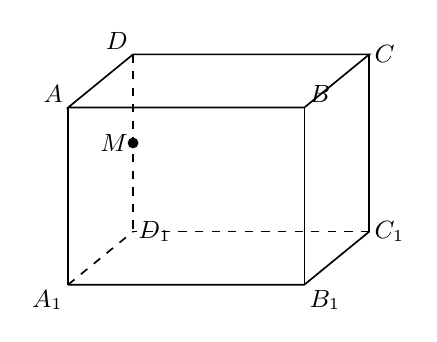
\begin{tikzpicture}[semithick, scale=1.5, every node/.style={inner sep=1.6pt, font=\small}]
  \coordinate (A) at (0,0);
  \coordinate (B) at (2,0);
  \coordinate (C) at (2.55,0.45);
  \coordinate (D) at (0.55,0.45);
  \coordinate (A1) at (0,-1.5);
  \coordinate (B1) at (2,-1.5);
  \coordinate (C1) at (2.55,-1.05);
  \coordinate (D1) at (0.55,-1.05);
  \coordinate (M) at (0.55,-0.3);

  \draw (A) -- (B) -- (C) -- (D) -- cycle;
  \draw (A) -- (A1);
  \draw (B) -- (B1);
  \draw (C) -- (C1);
  \draw (A1) -- (B1) -- (C1);
  \draw[dashed] (C1) -- (D1);
  \draw[dashed] (A1) -- (D1);
  \draw[dashed] (D) -- (D1);
  \fill (M) circle (1.3pt);

  \node[above left] at (A) {$A$};
  \node[above right] at (B) {$B$};
  \node[right] at (C) {$C$};
  \node[above left] at (D) {$D$};
  \node[below left] at (A1) {$A_1$};
  \node[below right] at (B1) {$B_1$};
  \node[right] at (C1) {$C_1$};
  \node[right] at (D1) {$D_1$};
  \node[left] at (M) {$M$};
\end{tikzpicture}
\end{center}
\nopagebreak[4]
\Needspace{0.4\textheight}
\end{question}
\endgroup
\begingroup
\renewenvironment{question}{\Needspace{0.5\textheight}}{}
\begin{question}
\gkti{12}四位同学在同一个坐标系中分别选定了一个适当的区间，各自作出三个函数 $y=\sin2x$，$y=\sin\left(x+\dfrac\pi6\right)$，$y=\sin\left(x-\dfrac\pi3\right)$ 的图象如下。结果发现其中有一位同学作出的图象有错误，那么有错误的图象是（　）
\nopagebreak[4]
\begin{center}% 2010 年江西卷文科第 12 题：四个图象选项（A）—（D）。
% 来源 PDF：普通高考/2010/2010江西文.pdf，SHA-256 c8c86a7272df02211069e27098dcaf04a5cd8af9a9b4d54ffd14a8eb91347af3。
% 原页：第 1 页（A3 三栏）第 3 栏中部，书页码 609。
% 题设三条曲线：y=sin2x（周期 π）、y=sin(x+π/6)、y=sin(x−π/3)（后两条周期 2π，
%   相位差 π/2）；前者的频率是后两条的两倍，同区间内波峰数约为两倍。
% 重绘依据：原页每幅仅约 4cm 宽、曲线在上边框被裁切，逐像素判读不可靠，故本图为
%   按题设关系绘制的示意图：A、B、D 三幅中 sin2x 呈二倍频、两条慢曲线相差四分之一
%   周期；C 幅三条曲线同频（无二倍频），即错误项。已在 PROGRESS 登记。
% 实现说明：TikZ 的 plot 以度为角度单位，\x 取 0..720 度并线性映射到面板宽度，
%   正弦用 (\x) 度计算，避免把弧度误当角度。
\begin{tikzpicture}[semithick]
  \def\w{4.6}       % 面板宽 (cm)
  \def\hh{1.5}      % 面板高 (cm)
  \def\amp{0.62}    % 振幅 (cm)
  \def\xscale{0.0063889}  % cm/度 = 4.6/720
  % 正确画法：#1 为整体相位平移（度）
  \newcommand{\goodpanel}[1]{%
    % y = sin 2x ：720 度内四个波峰
    \draw[thick] plot[domain=0:720,samples=361]
      ({\x*\xscale},{\amp*sin(2*\x+#1)});
    % y = sin(x + pi/6)：三十度为 30 度相位
    \draw[thick] plot[domain=0:720,samples=241]
      ({\x*\xscale},{\amp*sin(\x+30+#1)});
    % y = sin(x - pi/3)：-60 度相位，与上一条相差 90 度
    \draw[thick] plot[domain=0:720,samples=241]
      ({\x*\xscale},{\amp*sin(\x-60+#1)});
  }
  % 错误画法：三条曲线同为慢频（无二倍频），相位各不相同
  \newcommand{\badpanel}{%
    \draw[thick] plot[domain=0:720,samples=241]
      ({\x*\xscale},{\amp*sin(\x+20)});
    \draw[thick] plot[domain=0:720,samples=241]
      ({\x*\xscale},{\amp*sin(\x+110)});
    \draw[thick] plot[domain=0:720,samples=241]
      ({\x*\xscale},{\amp*sin(\x+200)});
  }
  % (A)
  \begin{scope}
    \draw (0,-\hh/2) rectangle (\w,\hh/2);
    \goodpanel{90}
    \node at (\w/2,-\hh/2-0.35) {（A）};
  \end{scope}
  % (B)
  \begin{scope}[shift={(5.5,0)}]
    \draw (0,-\hh/2) rectangle (\w,\hh/2);
    \goodpanel{150}
    \node at (\w/2,-\hh/2-0.35) {（B）};
  \end{scope}
  % (C) 错误项
  \begin{scope}[shift={(0,-2.5)}]
    \draw (0,-\hh/2) rectangle (\w,\hh/2);
    \badpanel
    \node at (\w/2,-\hh/2-0.35) {（C）};
  \end{scope}
  % (D)
  \begin{scope}[shift={(5.5,-2.5)}]
    \draw (0,-\hh/2) rectangle (\w,\hh/2);
    \goodpanel{210}
    \node at (\w/2,-\hh/2-0.35) {（D）};
  \end{scope}
\end{tikzpicture}
\end{center}
\nopagebreak[4]
\end{question}
\endgroup
\gkpart{二、填空题}

\begin{question}
\gkti{13}已知向量 $\boldsymbol a$，$\boldsymbol b$ 满足 $|\boldsymbol b|=2$，$\boldsymbol a$ 与 $\boldsymbol b$ 的夹角为 $60^\circ$，则 $\boldsymbol b$ 在 $\boldsymbol a$ 上的投影是$\underline{\qquad}$。

\end{question}
\begin{question}
\gkti{14}将 $5$ 位志愿者分成 $3$ 组，其中两组各 $2$ 人，另一组 $1$ 人，分赴世博会的三个不同场馆服务，不同的分配方案有$\underline{\qquad}$种。（用数字作答）

\end{question}
\begin{question}
\gkti{15}点 $A(x_0,y_0)$ 在双曲线 $\dfrac{x^2}{4}-\dfrac{y^2}{32}=1$ 的右支上，若点 $A$ 到右焦点的距离等于 $2x_0$，则 $x_0=$ $\underline{\qquad}$。

\Needspace{0.4\textheight}
\end{question}
\begingroup
\renewenvironment{question}{\Needspace{0.5\textheight}}{}
\begin{question}
\gkti{16}长方体 $ABCD-A_1B_1C_1D_1$ 的顶点均在同一个球面上，$AB=AA_1=1$，$BC=\sqrt2$，则 $A$，$B$ 两点间的球面距离为$\underline{\qquad}$。
\nopagebreak[4]
\begin{center}% 2010 年江西卷文科第 16 题：长方体 ABCD-A1B1C1D1。
% 来源 PDF：普通高考/2010/2010江西文.pdf，SHA-256 c8c86a7272df02211069e27098dcaf04a5cd8af9a9b4d54ffd14a8eb91347af3。
% 原页：第 1 页（A3 三栏）第 2 栏中部，书页码 609。
% 重绘依据：AB=AA1=1，BC=√2；A1D1、D1C1、DD1 为不可见棱，画虚线。
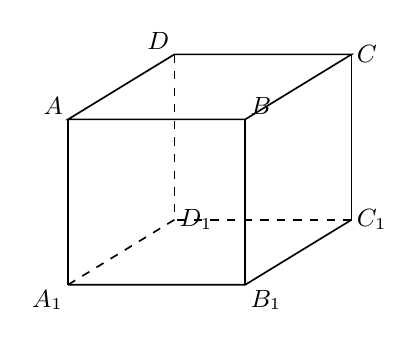
\begin{tikzpicture}[semithick, scale=1.5, every node/.style={inner sep=1.6pt, font=\small}]
  \coordinate (A) at (0,0);
  \coordinate (B) at (1.5,0);
  \coordinate (C) at (2.4,0.55);
  \coordinate (D) at (0.9,0.55);
  \coordinate (A1) at (0,-1.4);
  \coordinate (B1) at (1.5,-1.4);
  \coordinate (C1) at (2.4,-0.85);
  \coordinate (D1) at (0.9,-0.85);

  \draw (A) -- (B) -- (C) -- (D) -- cycle;
  \draw (A) -- (A1);
  \draw (B) -- (B1);
  \draw (C) -- (C1);
  \draw (A1) -- (B1) -- (C1);
  \draw[dashed] (C1) -- (D1);
  \draw[dashed] (A1) -- (D1);
  \draw[dashed] (D) -- (D1);

  \node[above left] at (A) {$A$};
  \node[above right] at (B) {$B$};
  \node[right] at (C) {$C$};
  \node[above left] at (D) {$D$};
  \node[below left] at (A1) {$A_1$};
  \node[below right] at (B1) {$B_1$};
  \node[right] at (C1) {$C_1$};
  \node[right] at (D1) {$D_1$};
\end{tikzpicture}
\end{center}
\nopagebreak[4]
\end{question}
\endgroup
\gkpart{三、解答题}

\begin{question}
\gkti{17}设函数 $f(x)=6x^3+3(a+2)x^2+2ax$。

（1）若 $f(x)$ 的两个极值点为 $x_1$，$x_2$，且 $x_1x_2=1$，求实数 $a$ 的值；

（2）是否存在实数 $a$，使得 $f(x)$ 是 $(-\infty,+\infty)$ 上的单调函数？若存在，求出 $a$ 的值；若不存在，说明理由。

\end{question}
\begin{question}
\gkti{18}某迷宫有三个通道，进入迷宫的每个人都要经过一个智能门。首次到达此门，系统会随机（即等可能）为你打开一个通道。若是 $1$ 号通道，则需要 $1$ 小时走出迷宫；若是 $2$ 号、$3$ 号通道，则分别需要 $2$ 小时、$3$ 小时返回智能门。再次到达智能门时，系统会随机打开一个你未到过的通道，直至走出迷宫为止。

（1）求走出迷宫时恰好用了 $1$ 小时的概率；

（2）求走出迷宫的时间超过 $3$ 小时的概率。

\end{question}
\begin{question}
\gkti{19}已知函数 $f(x)=(1+\cot x)\sin^2x-2\sin\left(x+\dfrac\pi4\right)\sin\left(x-\dfrac\pi4\right)$。

（1）若 $\tan\alpha=2$，求 $f(\alpha)$；

（2）若 $x\in\left[\dfrac\pi{12},\dfrac\pi2\right]$，求 $f(x)$ 的取值范围。

\Needspace{0.4\textheight}
\end{question}
\begingroup
\renewenvironment{question}{\Needspace{0.5\textheight}}{}
\begin{question}
\gkti{20}如图，$\triangle BCD$ 与 $\triangle MCD$ 都是边长为 $2$ 的正三角形，平面 $MCD\perp$ 平面 $BCD$，$AB\perp$ 平面 $BCD$，$AB=2\sqrt3$。

（1）求直线 $AM$ 与平面 $BCD$ 所成的角的大小；

（2）求平面 $ACM$ 与平面 $BCD$ 所成二面角的正弦值。
\nopagebreak[4]
\begin{center}% 2010 年江西卷文科第 20 题：两个共边正三角形 BCD、MCD 与垂线段 AB。
% 来源 PDF：普通高考/2010/2010江西文.pdf，SHA-256 c8c86a7272df02211069e27098dcaf04a5cd8af9a9b4d54ffd14a8eb91347af3。
% 原页：第 2 页（A3 三栏）第 1 栏中部，书页码 610。
% 重绘依据：△BCD 在底面，△MCD 与底面垂直并向上折起；AB⊥平面 BCD，AB=2√3；
%   AM、CM、DM 为实线，BM、BD 在遮挡处按原页保留实线，BC 与 MD 用虚线。
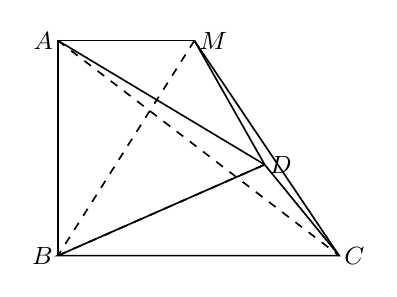
\begin{tikzpicture}[semithick, scale=1.05, every node/.style={inner sep=1.6pt, font=\small}]
  \coordinate (B) at (0,0);
  \coordinate (C) at (3.4,0);
  \coordinate (D) at (2.5,1.1);
  \coordinate (A) at (0,2.6);
  \coordinate (M) at (1.65,2.6);

  \draw (B) -- (C) -- (D) -- cycle;
  \draw (B) -- (A) -- (M);
  \draw (M) -- (C);
  \draw (M) -- (D);
  \draw (A) -- (D);
  \draw[dashed] (A) -- (C);
  \draw[dashed] (B) -- (D);
  \draw[dashed] (M) -- (B);

  \node[left] at (A) {$A$};
  \node[left] at (B) {$B$};
  \node[right] at (C) {$C$};
  \node[right] at (D) {$D$};
  \node[right] at (M) {$M$};
\end{tikzpicture}
\end{center}
\nopagebreak[4]
\Needspace{0.4\textheight}
\end{question}
\endgroup
\begingroup
\renewenvironment{question}{\Needspace{0.5\textheight}}{}
\begin{question}
\gkti{21}如图，已知抛物线 $C_1:x^2+by=b^2$ 经过椭圆 $C_2:\dfrac{x^2}{a^2}+\dfrac{y^2}{b^2}=1$（$a>b>0$）的两个焦点。

（1）求椭圆 $C_2$ 的离心率；

（2）设 $Q(3,b)$，又 $M$，$N$ 为 $C_1$ 与 $C_2$ 不在 $y$ 轴上的两个交点，若 $\triangle QMN$ 的重心在抛物线 $C_1$ 上，求 $C_1$ 和 $C_2$ 的方程。
\nopagebreak[4]
\begin{center}% 2010 年江西卷文科第 21 题：抛物线 C1、椭圆 C2 与点 Q、M、N。
% 来源 PDF：普通高考/2010/2010江西文.pdf，SHA-256 c8c86a7272df02211069e27098dcaf04a5cd8af9a9b4d54ffd14a8eb91347af3。
% 原页：第 2 页（A3 三栏）第 2 栏上部，书页码 610。
% 重绘依据：C1:x^2+y=1（开口向下、顶点 (0,1)），C2:x^2/2+y^2=1；
%   M、N 为两者在 y 轴两侧的交点，位于 y=-1/2；Q(3,1) 在右上方。
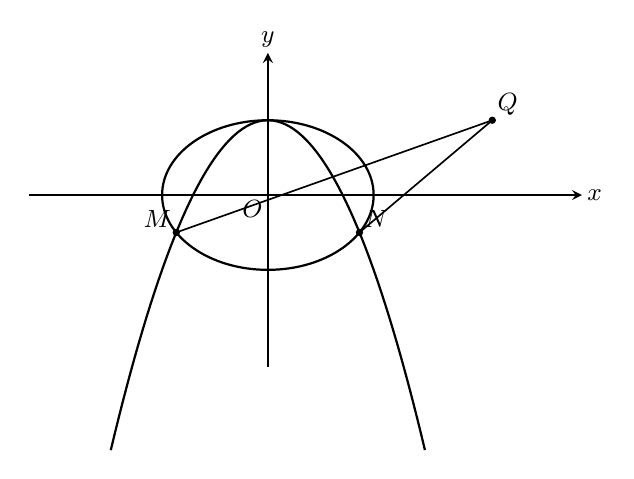
\begin{tikzpicture}[semithick, scale=0.95, every node/.style={inner sep=1.6pt, font=\small}]
  \draw[-stealth] (-3.2,0) -- (4.2,0) node[right] {$x$};
  \draw[-stealth] (0,-2.3) -- (0,1.9) node[above] {$y$};
  \draw[thick,domain=-2.1:2.1,samples=80] plot (\x,{1-(\x)*(\x)});
  \draw[thick] (0,0) ellipse (1.414 and 1);
  \fill (1.2247,-0.5) circle (1.4pt) node[above right] {$N$};
  \fill (-1.2247,-0.5) circle (1.4pt) node[above left] {$M$};
  \fill (3,1) circle (1.4pt) node[above right] {$Q$};
  \draw (3,1) -- (-1.2247,-0.5);
  \draw (3,1) -- (1.2247,-0.5);
  \node[below left] at (0,0) {$O$};
\end{tikzpicture}
\end{center}
\nopagebreak[4]
\end{question}
\endgroup
\begin{question}
\gkti{22}正实数数列 $\{a_n\}$ 中，$a_1=1$，$a_2=5$，且 $\{a_n^2\}$ 成等差数列。

（1）证明：数列 $\{a_n\}$ 中有无穷多项为无理数；

（2）当 $n$ 为何值时，$a_n$ 为整数，并求出使 $a_n<200$ 的所有整数项的和。

\end{question}